\chapter{Descripción de la realización}

\section{Método de desarrollo}

En el EDT del proyecto (Figura~\ref{fig:edt}) podemos ver cómo se realizará el proyecto, y cómo se hará la subdivisión de las tareas.

\begin{figure}
	\centering
	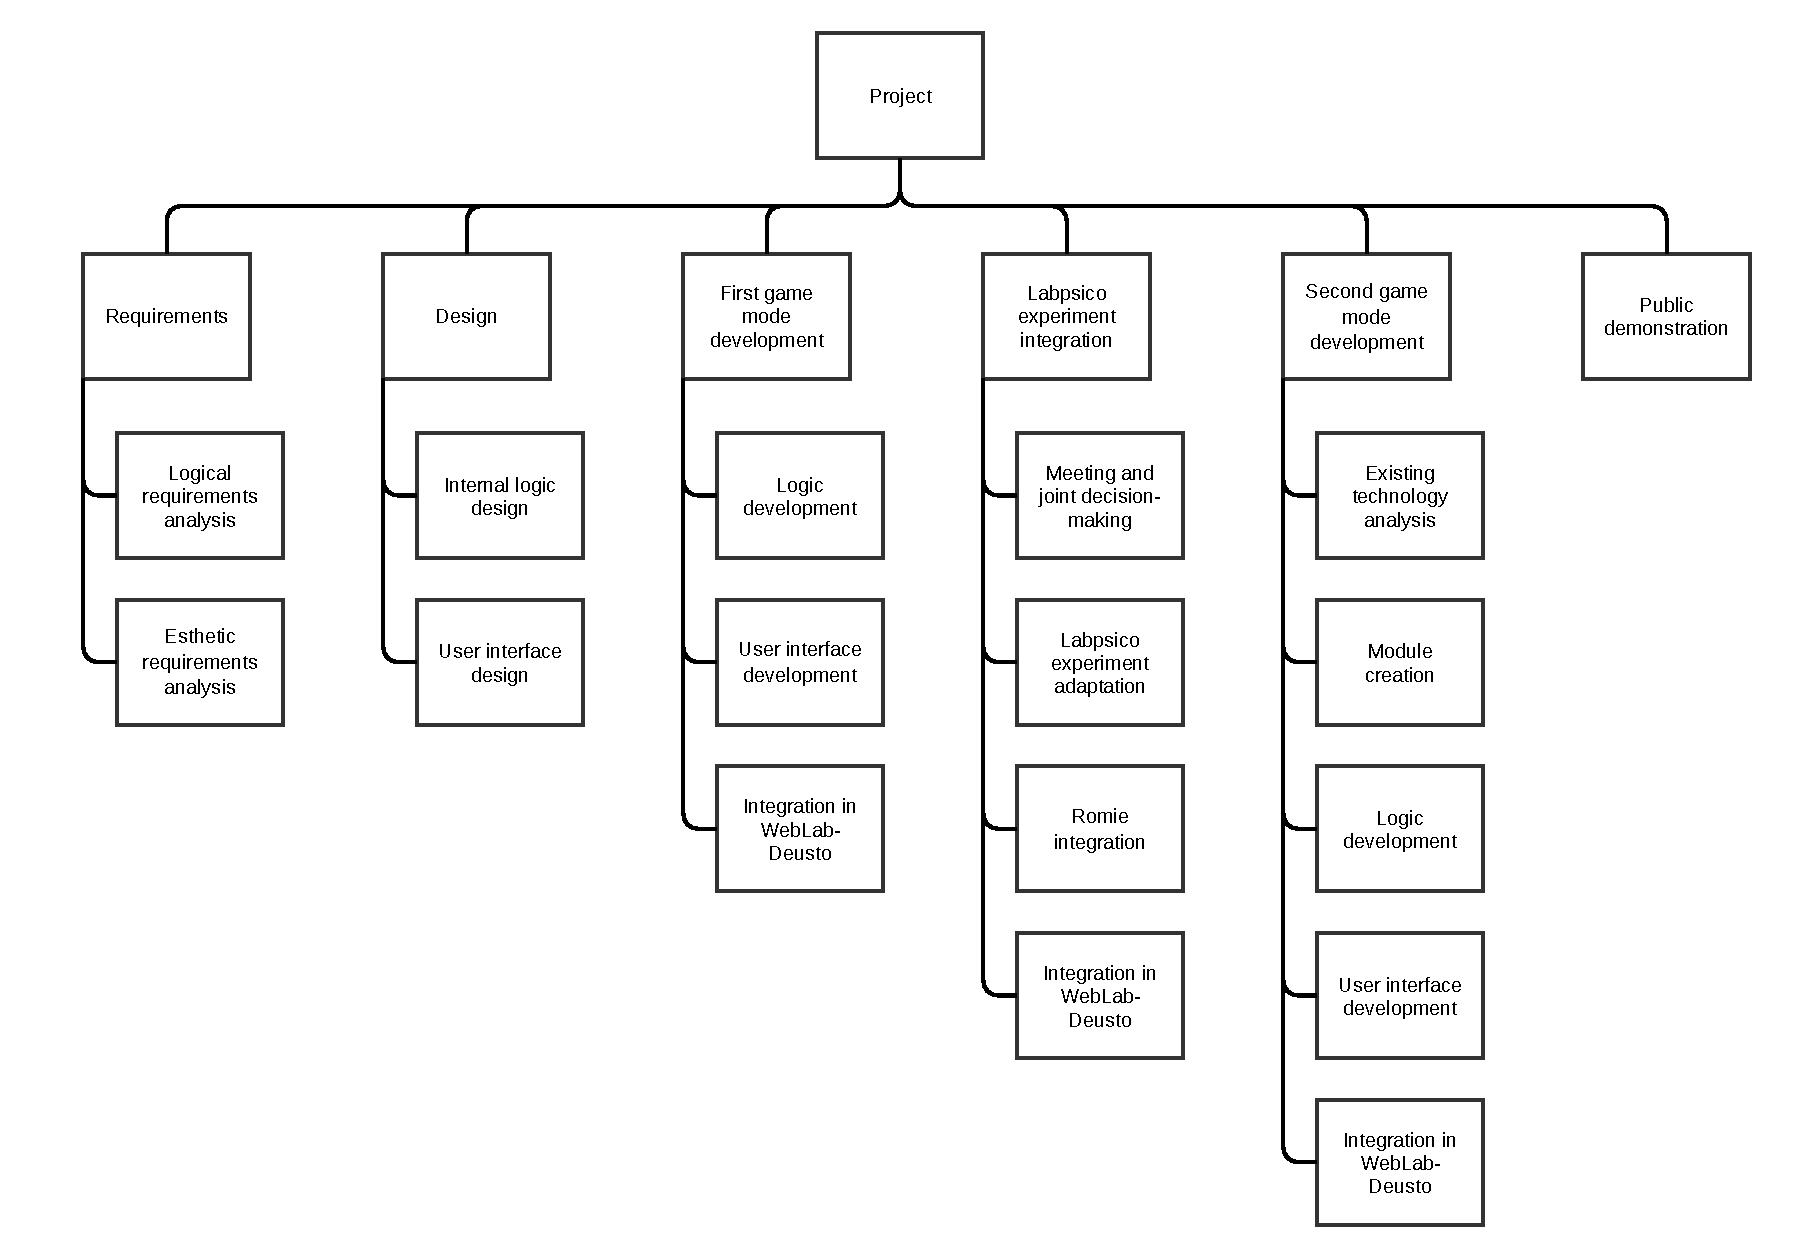
\includegraphics[height=\textwidth, angle=-90]{fig/edt}
	\caption{EDT del proyecto.}\label{fig:edt}
\end{figure}

Como se puede ver en el EDT, las fases del proyecto son las siguientes:

\begin{itemize}
\item \textbf{Requisitos}: Análisis de requisitos del proyecto, en el que se determinarán cuales
serán los requisitos funcionales y estéticos del proyecto.

\item \textbf{Diseño}: Exhaustivo diseño del proyecto, tanto funcional como estético, para definir
cómo será el producto final.

\item \textbf{Creación de la primera modalidad de juego}: Se creará el primer producto intermedio,
y se integrará con la plataforma Weblab-Deusto.

\item \textbf{Integración con el experimento de Labpsico}: Se integrará con la primera modalidad de
juego un experimento psicológico proporcionado por el laboratorio de psicología de Deusto, Labpsico.

\item \textbf{Creación de la segunda modalidad de juego}: Se creará la segunda modalidad de juego,
basada en la programación visual, para ayuda al aprendizaje de lógica computacional.

\item \textbf{Demostración pública}: Se demostrará públicamente con alumnos de primaria y secundaria
para comprobar la viabilidad y fiabilidad del proyecto.
\end{itemize}

\subsection{Productos intermedios}

Estos serán los productos intermedios de los que se compondrá el proyecto:

\begin{itemize}
\item \textbf{Primera modalidad de juego}: Un juego tipo trivial en el que el usuario moverá el
robot por un laberinto y responderá preguntas en lugares concretos.

\item \textbf{Modalidad con experimento de Labpsico}: El mismo juego de la primera modalidad de
juego,  precedido por una completa experiencia psicológica de lucha contra la pseudociencia.

\item \textbf{Segunda modalidad de juego}: Se creará una modalidad de juego que permitirá a los
usuarios programar acciones del robot y hacerlo moverse por el laberinto, con simples retos.
\end{itemize}

\section{Tareas principales}

\subsection{Requisitos}

\begin{itemize}
\item \textbf{T1 - Análisis de requisitos lógicos}: Se debe hacer un análisis detallado de todos los
requisitos funcionales de la plataforma, para poder hacer un posterior seguimiento y comprobar su
cumplimiento.

\item \textbf{T2 - Análisis de requisitos estéticos}: Se debe hacer un análisis detallado de todos
los requisitos estéticos de la plataforma, para poder hacer un posterior seguimiento y comprobar su
cumplimiento.
\end{itemize}

\subsection{Diseño}

\begin{itemize}
\item \textbf{T3 - Diseño de la lógica interna}: Se debe diseñar la lógica interna del robot y de la
plataforma de control del mismo, para hacerla accesible, simple y estable.

\item \textbf{T4 - Diseño de la interfaz}: Se debe hacer un diseño de la interfaz de la plataforma
pensando en el usuario final, para que el robot sea fácil de controlar.
\end{itemize}

\subsection{Creación de la primera modalidad de juego}

\begin{itemize}
\item \textbf{T5 - Creación de la lógica}: Se creará la lógica interna del juego de trivial pensando
siempre en la modularidad y extensibilidad.

\item \textbf{T6 - Creación de la interfaz}: Se creará una interfaz acorde con los estándares de
usabilidad, así como teniendo en cuenta el crédito a los patrocinadores del proyecto.

\item \textbf{T7 - Integración con Weblab-Deusto}: Se integrará la plataforma de juego con
Weblab-Deusto, haciendo uso de su API y sus laboratorios.
\end{itemize}

\subsection{Integración con el experimento de Labpsico}

\begin{itemize}
\item \textbf{T8 - Reunión y toma de decisiones conjunta}: Se hará una reunión con el laboratorio de
psicología de Deusto, Labpsico, en la que se definirá cómo integraremos su experimento con Romie, el
robot que se usará en este proyecto.

\item \textbf{T9 - Adaptación del experimento de Labpsico}: Se adaptará el experimento de Labpsico
para que tenga sentido en el marco de Romie.

\item \textbf{T10 - Integración con Romie}: Se integrará el experimento con la plataforma existente
de Romie, haciendo uso de la interfaz creada para la primera modalidad de juego.

\item \textbf{T11 - Integración con Weblab-Deusto}: Se integrará el nuevo juego con Weblab-Deusto
haciendo uso de sus sistemas de colas y prioridades.
\end{itemize}

\subsection{Creación de la segunda modalidad de juego}

\begin{itemize}
\item \textbf{T12 - Análisis de tecnologías existentes}: Se hará un análisis detallado de las
tecnologías existentes para la programación gráfica, y se decidirá cual será la usada en esta
modalidad.

\item \textbf{T13 - Creación de los módulos básicos}: Se crearán los módulos básicos para programar
el robot.

\item \textbf{T14 - Desarrollo de lógica}: Se desarrollará la lógica interna de la modalidad de
juego, y se decidirá cómo se puntuará.

\item \textbf{T15 - Desarrollo de la interfaz}: Se desarrollará una interfaz sencilla de usar y que
permita acceder a todas las funciones de esta modalidad de juego.

\item \textbf{T16 - Integración con Weblab-Deusto}: Se integrará esta modalidad de juego con
Weblab-Deusto y se hará uso de su sistema de colas y prioridades para compartir el robot.
\end{itemize}

\subsection{Demostración pública}

\begin{itemize}
\item \textbf{T17 - Demostración pública}: Se hará al menos una demostración pública del robot durante su desarrollo en la que estudiantes lo probarán y jugarán con el.
\end{itemize}

\section{Hojas de tareas}

\subsection{Tarea 1}

\begin{center}
	\begin{tabular}{!{\VRule[4pt]}p{200pt}!{\VRule[2pt]}p{100pt}!{\VRule[4pt]}}
		\specialrule{4pt}{0pt}{0pt}
		\multicolumn{2}{!{\VRule[4pt]}c!{\VRule[4pt]}}{\Large{\textbf{\MakeUppercase{Hoja de tareas}}}} \\
		\specialrule{2pt}{0pt}{0pt}
		\multicolumn{2}{!{\VRule[4pt]}l!{\VRule[4pt]}}{\textbf{Nombre:} Iban Eguia Moraza} \\
		\multicolumn{2}{!{\VRule[4pt]}l!{\VRule[4pt]}}{\textbf{Fecha:} 29 de marzo de 2015} \\
		\specialrule{2pt}{0pt}{0pt}
		\textbf{Identificación de Tarea :  T1} &  \textbf{Duración :  1 día} \\
		\specialrule{4pt}{0pt}{0pt}
	\end{tabular}
\end{center}

\clearpage

